% !TEX root = ../notes_template.tex

\chapter{테일러 급수와 로랑 급수}

이 장에서는 영역 $D$에 정의된 복소해석함수 $f$는 
$D$의 임의의 점에서 급수 전개가 가능하다는 근본적인 성질을 먼저 공부할 것이다.
다음 그림에서 왼쪽을 참고하라.
\begin{figure*}[h!]
\begin{center}
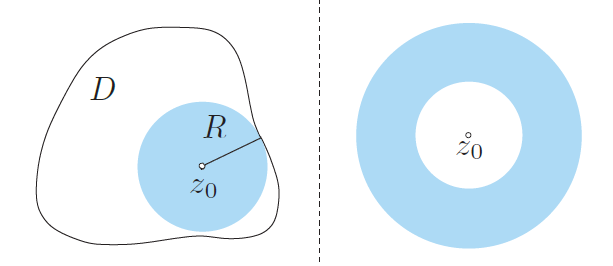
\includegraphics[width=0.5\textwidth]{./SaltChapter/fig-4-0-1}
\end{center}
\end{figure*}
\[
\text{테일러 급수: } \sum_{n=0}^\infty c_n(z-z_0)^n 
\quad
\text{로랑 급수: } \sum_{n\in \mathbb Z} c_n(z-z_0)^n 
\]

즉, 각각의 $z_0 \in D$에 대하여 다음을 만족하는 $R>0$이 존재한다.
\[
f(z) = \sum_{n=0}^\infty c_n(z-z_0)^n, \quad |z-z_0| <R.
\]
역으로,  적당한 $R$에 대하여 $|z-z_0|<R$을 만족하는 두 개 이상의 점에서 급수
\[
\sum_{n=0}^\infty c_n(z-z_0)^n
\]
가 수렴하면 $|z-z_0|<R$에서 복소해석함수이다.
이를 보이는 과정에서 복소해석함수에 대한 근본적인 성질들을 증명할 것이다.
\begin{itemize}
\item[(1)] (일반화된) 코시 적분공식과 코시 부등식
\item[(2)] 해의 분류와 항등정리
\item[(3)] 최대절대값정리
\end{itemize}

이 장의 후반부에서는
급수와 유사하지만 $z-z_0$ 항의 지수를 음의 정수까지 확장한
로랑 급수를 공부할 것이다.
이는 원환(특히 뚫린 원판)에 정의된 복소해석함수를 연구하는데 특히 유용하다,
앞의 그림에서 오른쪽을 참고하라.
끝으로 로랑 급수는 ``특이점''의 분류와 실함수 적분의 계산에도 유용함을 살펴볼 것이다.

\section{급수}

실수열의 경우와 유사하게 주어진
복소수열 $(a_n)_{n\in\mathbb N}$에 대하여
부분합 수열 $(s_n)_{n\in\mathbb N}$을 만들 수 있다.
\begin{align*}
s_1 &:= a_1, \\
s_2 &:= a_1 + a_2, \\
s_3 &:= a_1 + a_2 + a_3, \\
& \vdots
\end{align*}

\begin{salt_definition} \label{def-4-1}
\
\begin{itemize}
\item[(1)] 급수 
\item[(2)] 
\item[(3)] 
\end{itemize}
\end{salt_definition}










